\documentclass[border=12pt]{standalone}
\usepackage{tikz}
\usepackage{pgfplots}
\usepackage{amsmath,amssymb}
\usepackage[T1]{fontenc}
\usepackage{lmodern}
\usepackage{xcolor}
\usetikzlibrary{arrows.meta,positioning,shapes.geometric,calc,fit,matrix,backgrounds}
\pgfplotsset{compat=1.18}
\definecolor{ink}{HTML}{17202A}
\definecolor{blue}{HTML}{2463EB}
\definecolor{bluefill}{HTML}{EDF3FF}
\definecolor{green}{HTML}{16804A}
\definecolor{greenfill}{HTML}{EAF7EF}
\definecolor{amber}{HTML}{B56800}
\definecolor{amberfill}{HTML}{FFF4D8}
\definecolor{red}{HTML}{B42318}
\definecolor{redfill}{HTML}{FDEDEC}
\definecolor{purple}{HTML}{6B46C1}
\definecolor{purplefill}{HTML}{F2EDFF}
\definecolor{gray}{HTML}{667085}
\definecolor{light}{HTML}{F4F6F8}
\definecolor{linegray}{HTML}{CBD2D9}
\tikzset{
  every node/.style={font=\sffamily},
  box/.style={draw=ink, rounded corners=3pt, line width=1.1pt, fill=white, align=center, inner xsep=9pt, inner ysep=7pt, font=\sffamily\small},
  bluebox/.style={box, fill=bluefill, draw=blue},
  greenbox/.style={box, fill=greenfill, draw=green},
  amberbox/.style={box, fill=amberfill, draw=amber},
  redbox/.style={box, fill=redfill, draw=red},
  purplebox/.style={box, fill=purplefill, draw=purple},
  ghost/.style={box, draw=linegray, fill=light, text=gray},
  title/.style={font=\sffamily\bfseries\Large, text=ink, align=center},
  subtitle/.style={font=\sffamily\small, text=gray, align=center},
  arrow/.style={-{Latex[length=3mm,width=2mm]}, line width=1.2pt, draw=ink},
  bluearrow/.style={-{Latex[length=3mm,width=2mm]}, line width=1.2pt, draw=blue},
  greenarrow/.style={-{Latex[length=3mm,width=2mm]}, line width=1.2pt, draw=green},
  redarrow/.style={-{Latex[length=3mm,width=2mm]}, line width=1.2pt, draw=red},
  dashedarrow/.style={-{Latex[length=3mm,width=2mm]}, line width=1pt, dashed, draw=gray},
  smalllabel/.style={font=\sffamily\scriptsize, text=gray, align=center},
}

\begin{document}
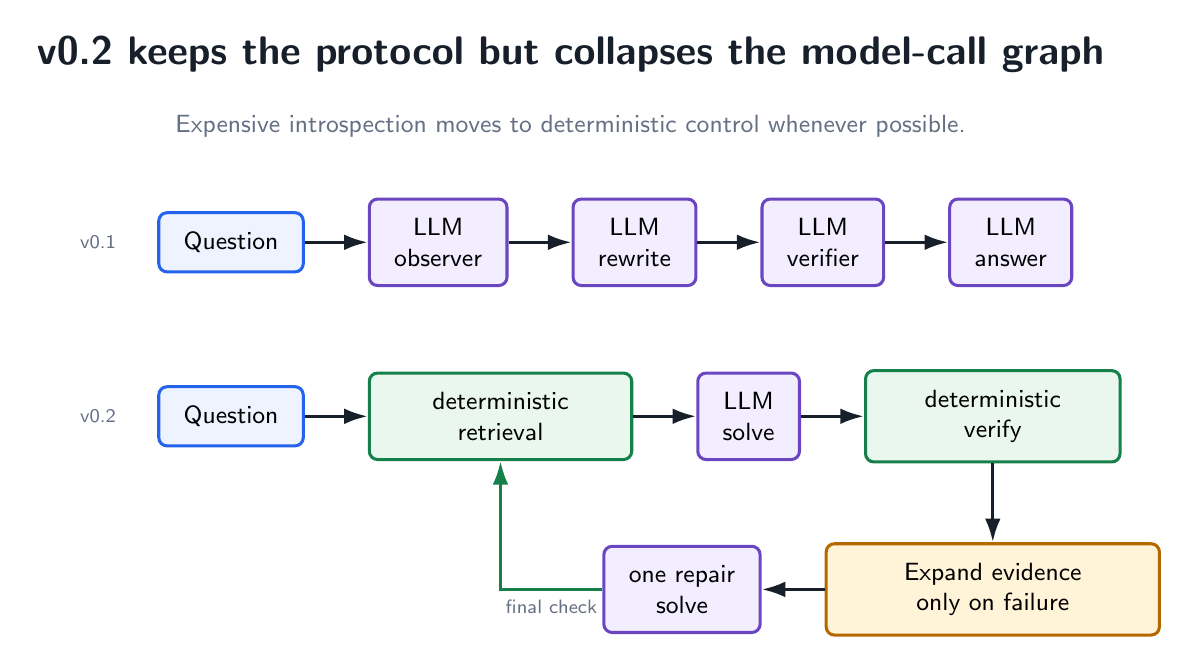
\begin{tikzpicture}[node distance=7mm and 8mm]
\node[title] (t) {v0.2 keeps the protocol but collapses the model-call graph};
\node[subtitle, below=3mm of t] (sub) {Expensive introspection moves to deterministic control whenever possible.};
\node[smalllabel, below=10mm of sub, xshift=-6.0cm] (l1) {v0.1};
\node[bluebox, right=4mm of l1] (q1) {Question};\node[purplebox,right=of q1](obs){LLM\\observer};\node[purplebox,right=of obs](rew){LLM\\rewrite};\node[purplebox,right=of rew](ver){LLM\\verifier};\node[purplebox,right=of ver](ans){LLM\\answer};
\draw[arrow](q1)--(obs);\draw[arrow](obs)--(rew);\draw[arrow](rew)--(ver);\draw[arrow](ver)--(ans);
\node[smalllabel, below=18mm of l1] (l2) {v0.2};
\node[bluebox, right=4mm of l2] (q2) {Question};\node[greenbox,right=of q2,text width=2.7cm](retr){deterministic\\retrieval};\node[purplebox,right=of retr](solve){LLM\\solve};\node[greenbox,right=of solve,text width=2.6cm](check){deterministic\\verify};
\draw[arrow](q2)--(retr);\draw[arrow](retr)--(solve);\draw[arrow](solve)--(check);
\node[amberbox, below=10mm of check,text width=3.6cm](exp){Expand evidence\\only on failure};\node[purplebox,left=of exp](repair){one repair\\solve};\draw[arrow](check)--(exp);\draw[arrow](exp)--(repair);\draw[greenarrow](repair.west)-|node[smalllabel,below,pos=.25]{final check}(retr.south);
\end{tikzpicture}
\end{document}
